\documentclass[conference]{IEEEtran}
\usepackage{cite}
\usepackage{amsmath,amssymb,amsfonts}
\usepackage{graphicx}
\usepackage{booktabs,tabularx}
\usepackage{xcolor}
\usepackage{microtype}
\usepackage{balance}
\usepackage[hidelinks]{hyperref}
\hypersetup{pdftitle={When Do Allocation Constraints Help? A Comparison of Five ETF Portfolios},
  pdfauthor={Rahul Sunilkumar},pdfsubject={Portfolio allocation research paper},
  pdfkeywords={asset allocation, portfolio constraints, transaction costs, risk parity}}
\graphicspath{{../figures/}{figures/}}
\date{Fall 2025}

\begin{document}
\raggedbottom

\title{When Do Allocation Constraints Help?\\
A Comparison of Five ETF Portfolios}
\author{\IEEEauthorblockN{Rahul Sunilkumar}
\IEEEauthorblockA{University of Virginia\\
Charlottesville, Virginia\\
Fall 2025}}
\maketitle

\begin{abstract}
An allocation rule can look attractive before limits and trading costs are applied. I compare equal weight, 60/40, minimum variance, maximum Sharpe, and risk parity across 18 exchange-traded funds, with monthly rebalancing and a 504-day estimation window. The evaluation runs from January 2009 through December 2024. With individual and asset-class caps and a cost of 10 basis points per dollar traded, minimum variance has the highest realized Sharpe ratio, 0.925, while equal weight has the highest compound annual return, 9.13 percent. Removing the caps changes the ranking: their effect depends on the rule and the performance measure. Maximum Sharpe trades the most and trails 60/40 even before costs. These results show how constraints change exposures and implementation costs in this sample; they do not establish a universally superior allocation rule.
\end{abstract}

\begin{IEEEkeywords}
asset allocation, portfolio constraints, transaction costs, minimum variance, risk parity
\end{IEEEkeywords}

\section{Introduction}
Portfolio optimization gives a precise answer to a problem built from uncertain estimates. A minimum variance portfolio uses an estimated covariance matrix; a maximum Sharpe portfolio also uses estimated returns. The mathematical objective is clear, but the allocation still has to work after the estimation window ends.

I wanted to see how much the answer changes when these rules face the same allocation limits and trading costs. The comparison includes two fixed-allocation baselines, equal weight and 60/40, and three rules that update their weights from recent returns. I keep the asset universe, estimation window, and rebalance schedule fixed, then compare portfolios with and without allocation caps and at three trading-cost levels.

There is a reason to take constraints seriously beyond treating them as an inconvenience. Jagannathan and Ma show how portfolio restrictions can alter the effect of sample covariance estimates and improve performance in their setting \cite{jagannathan}. That motivates this comparison, but does not establish what additional caps should do here: both of my cases already prohibit short selling.

The results made the distinction between an objective and an outcome useful. Minimum variance gives up growth for a smoother path in the main experiment. Maximum Sharpe does not produce the highest realized Sharpe. Caps help some measured outcomes and hurt others, sometimes by changing the portfolio's exposure rather than reducing its realized volatility.

\section{Data and Evaluation Design}
\subsection{A Fixed ETF Universe}
The data consist of adjusted daily closing prices downloaded from Yahoo Finance through \texttt{yfinance}, with automatic price adjustment enabled. The saved prices cover January 3, 2007 through December 30, 2024. The download's December 31 end date is exclusive. Simple returns are
\begin{equation}
 r_{i,t}=P_{i,t}/P_{i,t-1}-1.
\end{equation}
The resulting panel has 4,528 return dates and 18 ETFs, with no missing entries. Table~\ref{tab:universe} gives the groups used by the allocation constraints.

\begin{table}[t]
\caption{ETF Universe and Constraint Groups}
\label{tab:universe}
\centering
\small
\begin{tabularx}{\columnwidth}{@{}lX@{}}
\toprule
Asset class & Tickers \\
\midrule
U.S. equity & SPY, QQQ, IWM, DIA, XLF, XLE, XLK, XLV, XLU, XLP \\
International equity & EFA, EEM, EWJ \\
Fixed income & TLT, IEF \\
Commodity & GLD, USO \\
Real estate & VNQ \\
\bottomrule
\end{tabularx}
\end{table}

These are broad asset-class groups, even though the code calls the relevant parameter \texttt{sector\_cap}. The U.S. funds include overlapping broad-market and sector exposures. A cap on the mapped group is not a cap on every underlying company or economic risk. The fixed universe also conditions the result on these selected ETFs; it is not a historical universe-selection procedure.

\subsection{Estimation and Timing}
At each month-end, the three estimated rules use the latest $L=504$ daily returns, including the return at that close. Their annualized inputs are
\begin{align}
 \widehat\mu_t &= \frac{252}{L}\sum_{s=t-L+1}^{t}r_s,\\
 \widehat\Sigma_t &= \frac{252}{L-1}\sum_{s=t-L+1}^{t}
 (r_s-\bar r_t)(r_s-\bar r_t)^\top,
\end{align}
where $r_s$ is the vector of ETF returns and $\bar r_t$ is its window mean. There is no covariance shrinkage or separate expected-return model.

Rebalancing uses the last available trading day of each month. New target weights earn returns beginning on the following trading day; the return used to fit a target is never earned by that new target. Execution is assumed possible at the observed close, without an execution delay or market-impact model.

The first eligible rebalance is January 30, 2009. All reported strategies share 4,006 evaluation dates through December 30, 2024 and 191 rebalances, including initial entry. The first evaluation date records entry cost and zero gross return. The earlier observations are used for estimation, so this is not a full test of the 2008 financial crisis.

\subsection{The Two Constraint Sets}
Let $w$ be a vector of target weights and $G$ a group in Table~\ref{tab:universe}. The main experiment requires
\begin{equation}
 \begin{gathered}
 \mathbf{1}^\top w=1,\qquad 0\leq w_i\leq0.25,\\
 \sum_{i\in G}w_i\leq0.40\quad\text{for each }G.
 \end{gathered}
 \label{eq:caps}
\end{equation}
The comparison removes the 25\% individual and 40\% group caps, retaining nonnegative weights that sum to one. I call it \emph{long only without caps}, rather than unconstrained. Both caps change together, so the experiment does not isolate their separate effects. These restrictions apply to targets at rebalance; weights drift between trades and can subsequently exceed a target cap.

\section{Allocation Rules}
All five rules use the same applicable constraint set. The fixed-allocation rules must also be made feasible, which changes the meaning of their names under caps.

\subsection{Equal Weight and 60/40}
For equal weight, the initial target is $q_i=1/18$. The implemented allocation solves
\begin{equation}
 \min_w\sum_i(w_i-q_i)^2
 \label{eq:projection}
\end{equation}
subject to the portfolio constraints. Without caps this gives literal equal weights. With caps, the ten U.S. equity ETFs cannot jointly receive $10/18=55.56\%$. Their target becomes 4\% each, while each of the eight other ETFs receives 7.5\%. Thus the main experiment's ``equal weight'' is the closest feasible allocation to equal weight, not equal exposure across funds or asset classes.

The 60/40 target gives 60\% equally to 14 equity ETFs, including VNQ, and 40\% equally to TLT and IEF. Commodities receive zero. It minimizes the same squared distance while enforcing both sleeve totals. Under caps, the class targets are 40\% U.S. equity, 15\% international equity, 5\% real estate, and 40\% bonds. These two baselines do not estimate returns or covariance to choose weights, although they rebalance on the same dates as the other rules.

\subsection{Minimum Variance}
Minimum variance chooses
\begin{equation}
 \min_w w^\top\widehat\Sigma_t w.
\end{equation}
This uses estimated joint variability and makes no expected-return forecast. Its objective is low estimated variance, not high growth or a high return-to-risk ratio. Restricting the feasible set cannot lower the minimum of this same estimated objective. Whether restrictions improve subsequent performance is a separate empirical question.

\subsection{Maximum Sharpe}
Maximum Sharpe chooses
\begin{equation}
 \max_w\frac{w^\top\widehat\mu_t}
 {\sqrt{w^\top\widehat\Sigma_t w}}.
\end{equation}
The assumed risk-free rate is zero, matching the evaluation metric. This rule optimizes a ratio estimated from the past 504 days. It does not directly optimize the Sharpe ratio that will be measured over the subsequent backtest, nor does its objective charge for moving from the current allocation to the new one.

\subsection{Risk Parity}
For covariance matrix $\widehat\Sigma_t$, asset $i$ contributes $w_i(\widehat\Sigma_t w)_i$ to portfolio variance. Its share is
\begin{equation}
 s_i(w)=\frac{w_i(\widehat\Sigma_t w)_i}
 {w^\top\widehat\Sigma_t w},\qquad \sum_i s_i(w)=1.
\end{equation}
The same shares arise from volatility risk contributions. Following the equal-risk-contribution idea \cite{maillard}, the implemented rule minimizes
\begin{equation}
 \min_w\sum_i\left(s_i(w)-\frac{1}{18}\right)^2.
\end{equation}
Equal risk shares need not correspond to equal capital weights. Caps can also prevent exact equality, so ``risk parity'' here means the constrained squared-error objective, not a guarantee that every fitted contribution is identical.

All allocations use SLSQP with an equal-weight starting point, a maximum of 500 iterations, and an objective tolerance of $10^{-10}$. The implementation checks the returned constraints and stops on a failed optimization. Portfolio-variance denominators are floored at $10^{-12}$. Numerical success is not a global-optimality certificate for the nonlinear objectives.

\begin{table*}[t]
\caption{Main Results: Allocation Caps and 10 bps per Dollar Traded}
\label{tab:main}
\centering
\small
\begin{tabular}{@{}lrrrrrr@{}}
\toprule
Rule & Net CAGR (\%) & Annual vol. (\%) & Net Sharpe & Max. drawdown (\%) & Mean turnover (\%) & Cost drag (bps) \\
\midrule
Equal weight & 9.13 & 13.19 & 0.729 & 27.78 & 3.43 & 4.50 \\
60/40 & 8.51 & 9.85 & 0.879 & 21.99 & 3.11 & 4.05 \\
Minimum variance & 6.55 & 7.14 & 0.925 & 18.03 & 6.72 & 8.61 \\
Maximum Sharpe & 7.29 & 9.61 & 0.780 & 24.68 & 25.22 & 32.56 \\
Risk parity & 8.86 & 10.75 & 0.844 & 22.00 & 5.52 & 7.22 \\
\bottomrule
\end{tabular}
\par\smallskip
\begin{minipage}{0.96\textwidth}
\footnotesize All rules cover January 30, 2009--December 30, 2024, with 4,006 daily observations and 191 rebalances. Turnover counts both purchases and sales and includes initial entry. Equal weight and 60/40 are the feasible baseline allocations described in Section III. Sharpe assumes a zero risk-free rate.
\end{minipage}
\end{table*}

\section{Returns, Costs, and Performance Measures}
Let $w^-_t$ denote weights entering day $t$. Before trading, the portfolio earns gross return $g_t=(w^-_t)^\top r_t$, and its weights drift to
\begin{equation}
 \widetilde w_{i,t}=\frac{w^-_{i,t}(1+r_{i,t})}{1+g_t}.
\end{equation}
On a rebalance date with new target $w^*_t$, traded notional as a fraction of wealth is
\begin{equation}
 U_t=\sum_i\left|w^*_{i,t}-\widetilde w_{i,t}\right|.
\end{equation}
This counts purchases and sales: selling 10\% and buying 10\% gives $U_t=20\%$. It is not the half-sum convention sometimes used for turnover. On non-rebalance dates, $U_t=0$.

If $k$ is the cost per dollar traded, net return is
\begin{equation}
 n_t=(1+g_t)(1-kU_t)-1.
 \label{eq:net}
\end{equation}
The main comparison uses $k=0.001$, or 10 basis points (bps). The sensitivity analysis uses 0, 10, and 25 bps with caps. Initial entry has $U_t=1$ and is charged; terminal liquidation is not. Targets apply to wealth remaining after cost. Because turnover is computed from weights before costs, this is a proportional-cost approximation, not a detailed cash-flow execution simulation.

For $T$ daily net returns with arithmetic mean $\bar n$ and sample standard deviation $s_n$, the reported measures are
\begin{align}
 \mathrm{CAGR} &= \left[\prod_{t=1}^{T}(1+n_t)\right]^{252/T}-1,\\
 \sigma_{\mathrm{ann}} &= \sqrt{252}\,s_n,\\
 \mathrm{Sharpe} &= \sqrt{252}\,\bar n/s_n.
\end{align}
The last expression follows the historical mean-to-variability calculation \cite{sharpe}, using zero as the cash benchmark. It is not an excess-return Sharpe relative to observed Treasury bill returns. The annualization is the usual square-root convention, without a serial-correlation adjustment.

Maximum drawdown is the largest proportional loss from a prior equity peak, reported as a positive loss magnitude. The initial capital value is included before entry cost. Mean turnover averages $U_t$ over rebalance dates, including entry. Cost drag is gross CAGR minus net CAGR, expressed in bps; it is not a sum of cash charges. The saved outputs also contain Sortino and Calmar ratios, but the discussion focuses on growth, volatility, Sharpe, drawdown, and trading.



\section{Results and Interpretation}
\subsection{A Better Ratio Is Not More Wealth}
Table~\ref{tab:main} gives the main comparison. Minimum variance has the highest net Sharpe, 0.925, the lowest annual volatility, 7.14\%, and the smallest maximum drawdown, 18.03\%. It also has the lowest net CAGR, 6.55\%. Equal weight has the highest CAGR, 9.13\%, but annual volatility is 13.19\% and maximum drawdown is 27.78\%.

Figure~\ref{fig:equity} shows the consequence for compounded wealth. One dollar grows to approximately \$4.01 under equal weight and \$2.74 under minimum variance. Minimum variance's higher ratio should not be read as a claim that it produced more money. The portfolios are fully invested without volatility targeting or leverage, so their differing risk levels remain part of the comparison.

The simple 60/40 rule is also a strong reference point: its 8.51\% CAGR and 0.879 Sharpe sit between the growth and stability extremes. Risk parity earns 8.86\% with greater volatility and a lower Sharpe than 60/40. Its maximum drawdown is almost identical, about 22\%. Equalizing estimated risk contributions is a distinct objective; it does not require superiority on these realized metrics.

\begin{figure}[t]
\centering
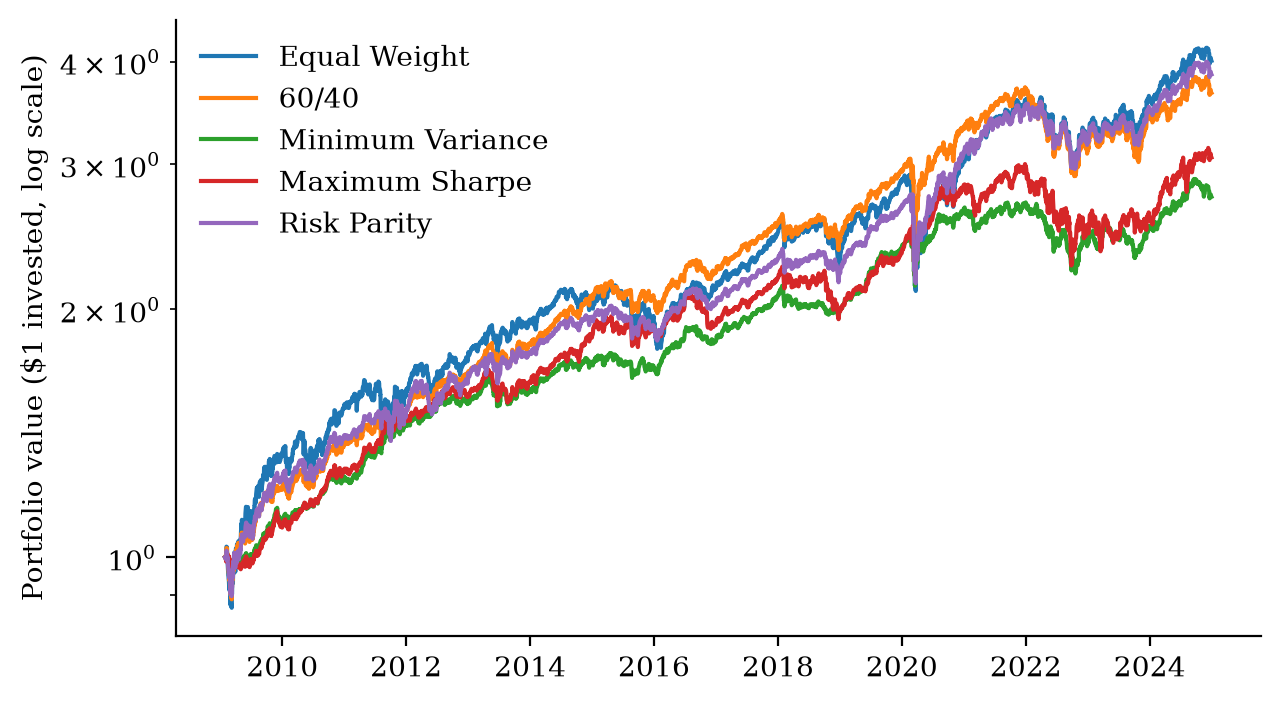
\includegraphics[width=\columnwidth]{equity.png}
\caption{Net wealth under caps and 10 bps trading cost. The logarithmic axis shows proportional growth. A higher realized Sharpe does not imply greater terminal wealth when portfolios operate at different risk levels.}
\label{fig:equity}
\end{figure}

\subsection{Caps Change the Portfolio, Not Just the Optimizer}
Table~\ref{tab:caps} compares realized Sharpe ratios with the same 10 bps cost. Caps raise minimum variance from 0.793 to 0.925 and maximum Sharpe from 0.721 to 0.780. They lower equal weight and 60/40, while risk parity changes only slightly. There is no common direction across the five rules.

\begin{table}[t]
\caption{Net Sharpe With and Without Allocation Caps}
\label{tab:caps}
\centering
\small
\begin{tabular}{@{}lrr@{}}
\toprule
Rule & Long only, no caps & With caps \\
\midrule
Equal weight & 0.781 & 0.729 \\
60/40 & 0.898 & 0.879 \\
Minimum variance & 0.793 & 0.925 \\
Maximum Sharpe & 0.721 & 0.780 \\
Risk parity & 0.842 & 0.844 \\
\bottomrule
\end{tabular}
\end{table}

Minimum variance is particularly revealing. Its mean bond target across rebalances falls from 74.92\% without caps to 38.90\% with caps. Net CAGR rises from 4.12\% to 6.55\%, but volatility also rises from 5.27\% to 7.14\%. The Sharpe improvement therefore accompanies more realized volatility, not less. The caps force a broader allocation away from a heavy bond position, changing both the return and risk profile. This is an observed exposure shift, not proof that covariance estimation became more accurate.

Risk parity shows a different tradeoff. Caps reduce its CAGR from 10.55\% to 8.86\% and its volatility from 12.91\% to 10.75\%, leaving Sharpe nearly unchanged. Maximum drawdown falls from 27.89\% to 22.00\%. A reader focused only on Sharpe would miss that change in the investment experience.

The baseline results also matter. Equal weight without caps assigns 55.56\% to the U.S. equity group simply because that group contains ten of the eighteen ETFs. Imposing the 40\% cap changes this static allocation even though there is no estimated covariance to stabilize. Its lower constrained CAGR, 9.13\% versus 10.49\%, cannot be explained as an optimizer becoming more or less accurate. It comes from a different allocation and its resulting returns and trades.

\subsection{Trading Costs Amplify an Existing Gap}
Maximum Sharpe trades 25.22\% of wealth per rebalance on average, compared with 3.11\% for 60/40, roughly eight times as much. At 10 bps, its CAGR drag is 32.56 bps versus 4.05 bps for 60/40. Figure~\ref{fig:cost} shows the greater sensitivity of its realized Sharpe to the cost assumption.

\begin{figure}[t]
\centering
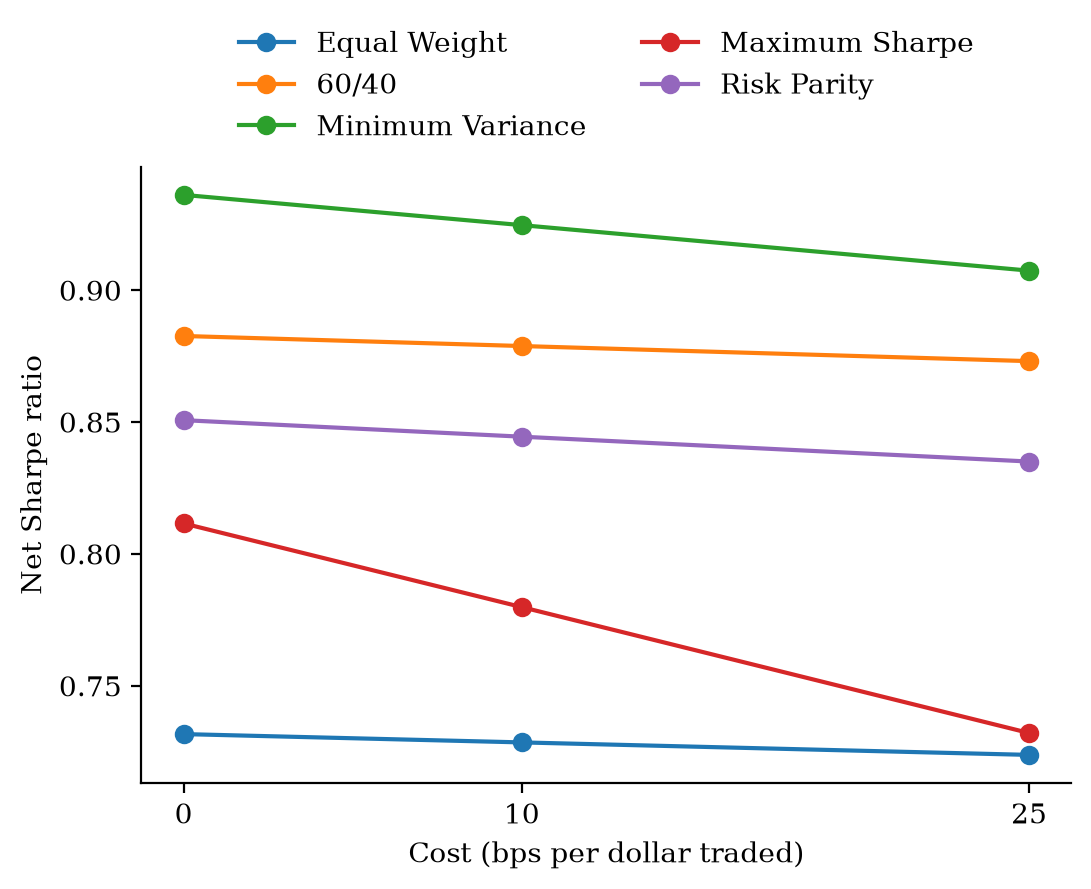
\includegraphics[width=\columnwidth]{cost_sensitivity.png}
\caption{Realized Sharpe at the three tested trading-cost levels, with allocation caps. Connecting lines are visual guides. Costs change net wealth but do not enter the allocation objectives, so the targets do not adapt to higher costs.}
\label{fig:cost}
\end{figure}

At zero cost, maximum Sharpe achieves 0.812, already below 60/40's 0.883 and minimum variance's 0.936. At 25 bps, its Sharpe falls to 0.732 and its CAGR to 6.80\%, compared with 7.61\% gross CAGR. Costs worsen the outcome but do not explain the original ranking. The ordering of the five capped rules by Sharpe is unchanged at all three tested cost levels.

It is tempting to attribute this entirely to noisy mean estimates. That is plausible because maximum Sharpe uses estimated means and repeatedly changes its allocation. The experiment does not isolate this mechanism, however. It compares complete allocation rules, not alternative mean estimators with everything else held constant. What the outputs directly establish is high turnover and weaker realized performance than several simpler rules.

Caps do reduce maximum Sharpe's mean turnover from 33.15\% to 25.22\%, but they also change exposure. Its improved full-period Sharpe coexists with a larger maximum drawdown, 24.68\% versus 22.83\%. Even for the rule most sensitive to trading, the benefit of caps depends on which outcome matters.

\subsection{The 2020 Window Qualifies the Overall Ranking}
Figure~\ref{fig:covid} retains the existing January--June 2020 comparison, rebased to the end of 2019. During this window, capped maximum Sharpe reaches a low 6.53\% below its starting value and finishes June up 10.70\%. Minimum variance reaches a low 9.79\% below the starting value and finishes up 3.54\%. These lows are relative to December 31 wealth, not peak-to-trough drawdowns.

\begin{figure}[t]
\centering
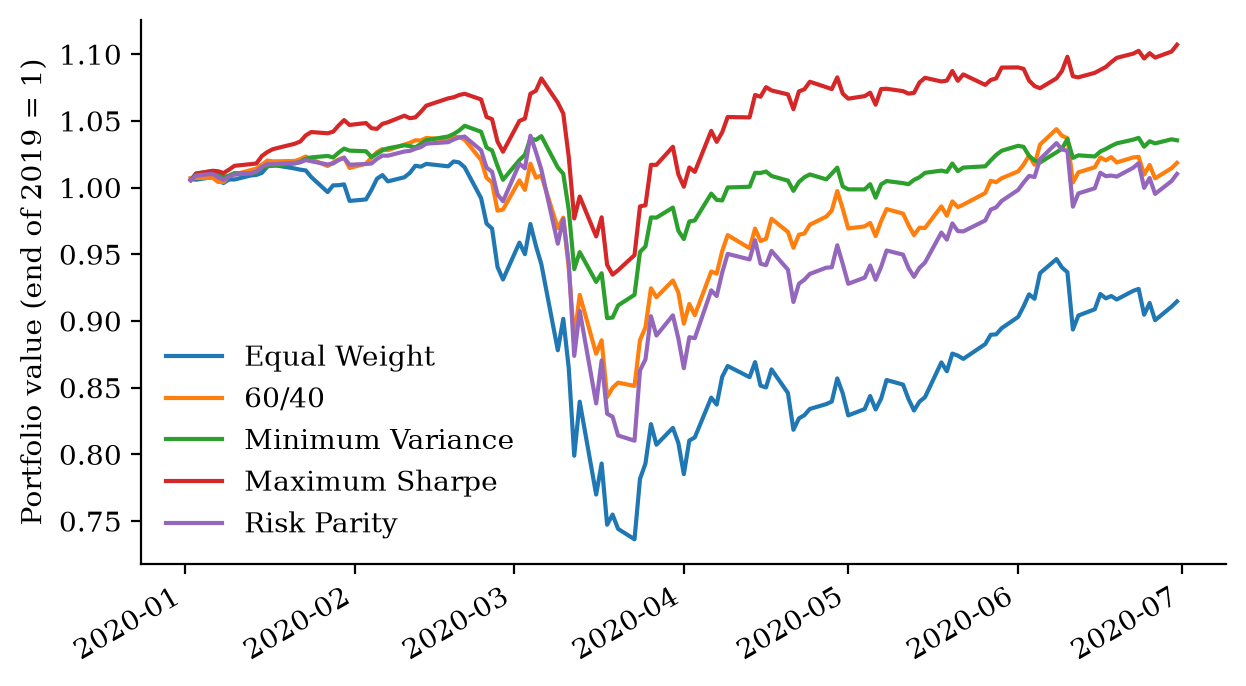
\includegraphics[width=\columnwidth]{covid_2020.png}
\caption{Capped portfolios over January--June 2020, net of 10 bps trading cost and rebased to end-2019 wealth. The selected window shows a different ordering from the full-period Sharpe comparison.}
\label{fig:covid}
\end{figure}

Thus maximum Sharpe's weaker full-period result does not mean that it performs poorly in every difficult interval. Conversely, a favorable six-month path does not establish crisis protection. This is one selected historical window using the same previously fitted sequence of allocations, not a separate stress-testing model or a repeated test across crises.

\section{Limits of the Comparison}
The study is a retrospective comparison of five implemented rules on one fixed ETF universe. The 504-day window, monthly schedule, and cap levels are held fixed; the results do not show that these are optimal choices. The sequential fitting prevents future returns from entering each estimation window, but there is no separate holdout for selecting the overall research design and no confidence interval or significance test for differences in performance.

The universe overlaps economically and uses broad fund labels. Consequently, more tickers or lower ticker weights do not by themselves demonstrate greater diversification of underlying risks. The caps also apply only at rebalance. Any interpretation as continuously enforced exposure limits would overstate what the code does.

The cost rates are uniform scenarios rather than asset-specific spread estimates. The backtest omits taxes, market impact, and execution delay, uses adjusted price histories, and assumes a zero risk-free rate. The reported Sharpe levels and even their ranking need not carry over to a comparison using observed cash returns. The numerical solver adds another limit: a successful local solve is evidence of a feasible implementation, not proof that every nonlinear allocation is globally best.

\section{Conclusion}
I began with the question of whether allocation constraints help portfolio rules work better after trading costs. In this sample, the answer depends on the rule and the measure. Minimum variance has the best constrained Sharpe and the smallest full-period drawdown, while equal weight builds the most wealth. Caps improve minimum variance's ratio while increasing its volatility, and risk parity's nearly unchanged ratio conceals a meaningful reduction in both growth and drawdown.

Maximum Sharpe makes the cost of implementation especially visible. It trades the most and loses the most CAGR to costs, but it already trails simpler rules before those costs are charged. Its favorable 2020 path also keeps the conclusion from becoming too broad. I would read these results as evidence that an allocation objective, its constraints, and its realized performance need to be examined separately, rather than as a recommendation to use one rule in every setting.

\section*{Reproducibility}
The code and paper are available in the project repository \cite{repository}. The paper uses the saved returns and analysis outputs in the project's \texttt{data/} and \texttt{results/} folders. Running \texttt{run\_analysis.py} produces the main, no-cap, and cost-sensitivity comparisons. Running \texttt{make\_plots.py} reads those outputs and saves PNG figures. The price download is handled by \texttt{fetch.py}; a later download may contain provider revisions. The existing synthetic checks in \texttt{test\_backtest.py} cover constraints, rebalance timing, drift, costs, metric definitions, risk parity on a diagonal covariance matrix, and future-data isolation. They verify implementation properties rather than the economic reliability of the results.

\balance
\begin{thebibliography}{4}
\bibitem{jagannathan}
R. Jagannathan and T. Ma, ``Risk reduction in large portfolios: Why imposing the wrong constraints helps,'' \emph{Journal of Finance}, vol. 58, no. 4, pp. 1651--1684, 2003. Working paper available: \url{https://www.nber.org/papers/w8922}.

\bibitem{maillard}
S. Maillard, T. Roncalli, and J. Teiletche, ``The properties of equally weighted risk contribution portfolios,'' \emph{Journal of Portfolio Management}, vol. 36, no. 4, pp. 60--70, 2010. Author manuscript available: \url{https://www.thierry-roncalli.com/download/erc.pdf}.

\bibitem{sharpe}
W. F. Sharpe, ``The Sharpe ratio,'' \emph{Journal of Portfolio Management}, vol. 21, no. 1, pp. 49--58, 1994. Available: \url{https://web.stanford.edu/~wfsharpe/art/sr/sr.htm}.
\bibitem{repository}
R. Sunilkumar, ``Allocation constraints,'' GitHub repository. [Online]. Available: \url{https://github.com/rahulsunilkumar/allocation-constraints}.
\end{thebibliography}
\end{document}
